\documentclass[a4paper,11pt]{article}
\usepackage[a4paper, margin=8em]{geometry}

% usa i pacchetti per la scrittura in italiano
\usepackage[french,italian]{babel}
\usepackage[T1]{fontenc}
\usepackage[utf8]{inputenc}
\frenchspacing 

% usa i pacchetti per la formattazione matematica
\usepackage{amsmath, amssymb, amsthm, amsfonts}

% usa altri pacchetti
\usepackage{gensymb}
\usepackage{hyperref}
\usepackage{standalone}

\usepackage{colortbl}

\usepackage{xstring}
\usepackage{karnaugh-map}

% imposta il titolo
\title{Appunti Reti Informatiche}
\author{Luca Seggiani}
\date{2025}

% imposta lo stile
% usa helvetica
\usepackage[scaled]{helvet}
% usa palatino
\usepackage{palatino}
% usa un font monospazio guardabile
\usepackage{lmodern}

\renewcommand{\rmdefault}{ppl}
\renewcommand{\sfdefault}{phv}
\renewcommand{\ttdefault}{lmtt}

% circuiti
\usepackage{circuitikz}
\usetikzlibrary{babel}

% testo cerchiato
\newcommand*\circled[1]{\tikz[baseline=(char.base)]{
            \node[shape=circle,draw,inner sep=2pt] (char) {#1};}}

% disponi il titolo
\makeatletter
\renewcommand{\maketitle} {
	\begin{center} 
		\begin{minipage}[t]{.8\textwidth}
			\textsf{\huge\bfseries \@title} 
		\end{minipage}%
		\begin{minipage}[t]{.2\textwidth}
			\raggedleft \vspace{-1.65em}
			\textsf{\small \@author} \vfill
			\textsf{\small \@date}
		\end{minipage}
		\par
	\end{center}

	\thispagestyle{empty}
	\pagestyle{fancy}
}
\makeatother

% disponi teoremi
\usepackage{tcolorbox}
\newtcolorbox[auto counter, number within=section]{theorem}[2][]{%
	colback=blue!10, 
	colframe=blue!40!black, 
	sharp corners=northwest,
	fonttitle=\sffamily\bfseries, 
	title=Teorema~\thetcbcounter: #2, 
	#1
}

% disponi definizioni
\newtcolorbox[auto counter, number within=section]{definition}[2][]{%
	colback=red!10,
	colframe=red!40!black,
	sharp corners=northwest,
	fonttitle=\sffamily\bfseries,
	title=Definizione~\thetcbcounter: #2,
	#1
}

% disponi codice
\usepackage{listings}
\usepackage[table]{xcolor}

\definecolor{codegreen}{rgb}{0,0.6,0}
\definecolor{codegray}{rgb}{0.5,0.5,0.5}
\definecolor{codepurple}{rgb}{0.58,0,0.82}
\definecolor{backcolour}{rgb}{0.95,0.95,0.92}

\lstdefinestyle{codestyle}{
		backgroundcolor=\color{black!5}, 
		commentstyle=\color{codegreen},
		keywordstyle=\bfseries\color{magenta},
		numberstyle=\sffamily\tiny\color{black!60},
		stringstyle=\color{green!50!black},
		basicstyle=\ttfamily\footnotesize,
		breakatwhitespace=false,         
		breaklines=true,                 
		captionpos=b,                    
		keepspaces=true,                 
		numbers=left,                    
		numbersep=5pt,                  
		showspaces=false,                
		showstringspaces=false,
		showtabs=false,                  
		tabsize=2
}

\lstdefinestyle{shellstyle}{
		backgroundcolor=\color{black!5}, 
		basicstyle=\ttfamily\footnotesize\color{black}, 
		commentstyle=\color{black}, 
		keywordstyle=\color{black},
		numberstyle=\color{black!5},
		stringstyle=\color{black}, 
		showspaces=false,
		showstringspaces=false, 
		showtabs=false, 
		tabsize=2, 
		numbers=none, 
		breaklines=true
}


\lstdefinelanguage{assembler}{ 
  keywords={AAA, AAD, AAM, AAS, ADC, ADCB, ADCW, ADCL, ADD, ADDB, ADDW, ADDL, AND, ANDB, ANDW, ANDL,
        ARPL, BOUND, BSF, BSFL, BSFW, BSR, BSRL, BSRW, BSWAP, BT, BTC, BTCB, BTCW, BTCL, BTR, 
        BTRB, BTRW, BTRL, BTS, BTSB, BTSW, BTSL, CALL, CBW, CDQ, CLC, CLD, CLI, CLTS, CMC, CMP,
        CMPB, CMPW, CMPL, CMPS, CMPSB, CMPSD, CMPSW, CMPXCHG, CMPXCHGB, CMPXCHGW, CMPXCHGL,
        CMPXCHG8B, CPUID, CWDE, DAA, DAS, DEC, DECB, DECW, DECL, DIV, DIVB, DIVW, DIVL, ENTER,
        HLT, IDIV, IDIVB, IDIVW, IDIVL, IMUL, IMULB, IMULW, IMULL, IN, INB, INW, INL, INC, INCB,
        INCW, INCL, INS, INSB, INSD, INSW, INT, INT3, INTO, INVD, INVLPG, IRET, IRETD, JA, JAE,
        JB, JBE, JC, JCXZ, JE, JECXZ, JG, JGE, JL, JLE, JMP, JNA, JNAE, JNB, JNBE, JNC, JNE, JNG,
        JNGE, JNL, JNLE, JNO, JNP, JNS, JNZ, JO, JP, JPE, JPO, JS, JZ, LAHF, LAR, LCALL, LDS,
        LEA, LEAVE, LES, LFS, LGDT, LGS, LIDT, LMSW, LOCK, LODSB, LODSD, LODSW, LOOP, LOOPE,
        LOOPNE, LSL, LSS, LTR, MOV, MOVB, MOVW, MOVL, MOVSB, MOVSD, MOVSW, MOVSX, MOVSXB,
        MOVSXW, MOVSXL, MOVZX, MOVZXB, MOVZXW, MOVZXL, MUL, MULB, MULW, MULL, NEG, NEGB, NEGW,
        NEGL, NOP, NOT, NOTB, NOTW, NOTL, OR, ORB, ORW, ORL, OUT, OUTB, OUTW, OUTL, OUTSB, OUTSD,
        OUTSW, POP, POPL, POPW, POPB, POPA, POPAD, POPF, POPFD, PUSH, PUSHL, PUSHW, PUSHB, PUSHA, 
				PUSHAD, PUSHF, PUSHFD, RCL, RCLB, RCLW, MOVSL, MOVSB, MOVSW, STOSL, STOSB, STOSW, LODSB, LODSW,
				LODSL, INSB, INSW, INSL, OUTSB, OUTSL, OUTSW
        RCLL, RCR, RCRB, RCRW, RCRL, RDMSR, RDPMC, RDTSC, REP, REPE, REPNE, RET, ROL, ROLB, ROLW,
        ROLL, ROR, RORB, RORW, RORL, SAHF, SAL, SALB, SALW, SALL, SAR, SARB, SARW, SARL, SBB,
        SBBB, SBBW, SBBL, SCASB, SCASD, SCASW, SETA, SETAE, SETB, SETBE, SETC, SETE, SETG, SETGE,
        SETL, SETLE, SETNA, SETNAE, SETNB, SETNBE, SETNC, SETNE, SETNG, SETNGE, SETNL, SETNLE,
        SETNO, SETNP, SETNS, SETNZ, SETO, SETP, SETPE, SETPO, SETS, SETZ, SGDT, SHL, SHLB, SHLW,
        SHLL, SHLD, SHR, SHRB, SHRW, SHRL, SHRD, SIDT, SLDT, SMSW, STC, STD, STI, STOSB, STOSD,
        STOSW, STR, SUB, SUBB, SUBW, SUBL, TEST, TESTB, TESTW, TESTL, VERR, VERW, WAIT, WBINVD,
        XADD, XADDB, XADDW, XADDL, XCHG, XCHGB, XCHGW, XCHGL, XLAT, XLATB, XOR, XORB, XORW, XORL},
  keywordstyle=\color{blue}\bfseries,
  ndkeywordstyle=\color{darkgray}\bfseries,
  identifierstyle=\color{black},
  sensitive=false,
  comment=[l]{\#},
  morecomment=[s]{/*}{*/},
  commentstyle=\color{purple}\ttfamily,
  stringstyle=\color{red}\ttfamily,
  morestring=[b]',
  morestring=[b]"
}

\lstset{language=assembler, style=codestyle}

% disponi sezioni
\usepackage{titlesec}

\titleformat{\section}
	{\sffamily\Large\bfseries} 
	{\thesection}{1em}{} 
\titleformat{\subsection}
	{\sffamily\large\bfseries}   
	{\thesubsection}{1em}{} 
\titleformat{\subsubsection}
	{\sffamily\normalsize\bfseries} 
	{\thesubsubsection}{1em}{}

% tikz
\usepackage{tikz}

% float
\usepackage{float}

% grafici
\usepackage{pgfplots}
\pgfplotsset{width=10cm,compat=1.9}

% disponi alberi
\usepackage{forest}

\forestset{
	rectstyle/.style={
		for tree={rectangle,draw,font=\large\sffamily}
	},
	roundstyle/.style={
		for tree={circle,draw,font=\large}
	}
}

% disponi algoritmi
\usepackage{algorithm}
\usepackage{algorithmic}
\makeatletter
\renewcommand{\ALG@name}{Algoritmo}
\makeatother

% disponi numeri di pagina
\usepackage{fancyhdr}
\fancyhf{} 
\fancyfoot[L]{\sffamily{\thepage}}

\makeatletter
\fancyhead[L]{\raisebox{1ex}[0pt][0pt]{\sffamily{\@title \ \@date}}} 
\fancyhead[R]{\raisebox{1ex}[0pt][0pt]{\sffamily{\@author}}}
\makeatother

\begin{document}
% sezione (data)
\section{Lezione del 08-10-25}

% stili pagina
\thispagestyle{empty}
\pagestyle{fancy}

% testo
\subsection{Confronto prestazionale fra CS e P2P}
Vediamo di valutare quale approccio, fra client-server e peer-to-peer, per un job semplice come un trasferimento di file \textit{minimizza} il \textbf{tempo di trasferimento}.

Poniamo di avere $N$ peer (o client, comunque $n$ host che vogliono ricevere il file) e un server che contiene il file (di dimensione $F$). All'istante in cui il file viene reso disponibile ogni peer richiede il file, e vogliamo minimizzare il tempo che passa affinché tutti lo abbiano ricevuto.

Sia $u_s$ la capacità di upload del server, $u_i$ la capacità di upload dell'$i$-esimo peer e $d_i$ la capacità di download dell'$i$-esimo peer.

\begin{itemize}
	\item Con l'approccio \textbf{client-server}, il server deve inviare $N$ copie del file di dimensione $F$, che con capacità di upload di $u_s$ dà un tempo minimo di $NF / u_s$.
		Ogni client deve quindi ricevere la sua copia del file, che con capacità di download di $d_i$ diventa $F / d_i$. Visto che il più lento è quello che pregiudica tuta la statistica, prendiamo la sua capacità di download come $d_\text{min}$ e rifiniamo il bound:
		$$
			T_{cs} \geq \max\left( \frac{NF}{u_s}, \frac{F}{d_\text{min}} \right)
		$$
		Notiamo che questo bound è $O(N)$.
	\item Con l'approccio \textbf{peer-to-peer}, il server dovrà inviare al minimo una copia del file, per cui il bound diventa $F / u_s$. Il client più lento sarà comunque un bottleneck, per cui c'è il termine $F / d_\text{min}$. A questo punto l'ultimo bound viene preso come il tempo impiegato a trasferire il file a tutti, se tutti distribuiscono, cioè $NF / (u_s + \sum u_i)$. Questo dà il bound:
		$$
		T_{p2p} \geq \max\left( \frac{F}{u_s}, \frac{F}{d_\text{min}}, \frac{NF}{u_s + \sum u_i} \right)
		$$
		Vediamo che il termine significativo è l'ultimo: il primo non dipende da $N$, mentre il secondo lo fa in maniera "lasca" (aumentando $N$ troveremo host più lenti, ma non linearmente e prima o poi stabilizzandoci).
		Il terzo termine dipende da $N$, ma ancora non linearmente.
		Posto $\bar{u}$ come la velocita media di upload dei peer, possiamo approssimare come:
		$$
		T_{p2p} \sim \frac{NF}{u_s + \sum_1^N u_i} \approx \frac{NF}{u_s + N \bar{u}}
		$$
		che per $N\rightarrow\infty$ è:
		$$
		\lim_{N\rightarrow \infty} \frac{NF}{u_s + N \bar{u}} = \frac{F}{\bar{u}}
		$$
		ammesso di conoscere $\bar{u}$.

		Abbiamo quindi che il bound è migliore rispetto a quello dell'approccio client-server, in quanto prima o poi converge ad un valore finito. 

\end{itemize}

\noindent
\begin{minipage}{\textwidth}
Concludiamo tracciando su un grafico l'andamento complessivo dei bound più svantaggiosi dei tempi di trasferimento:
\begin{center}
	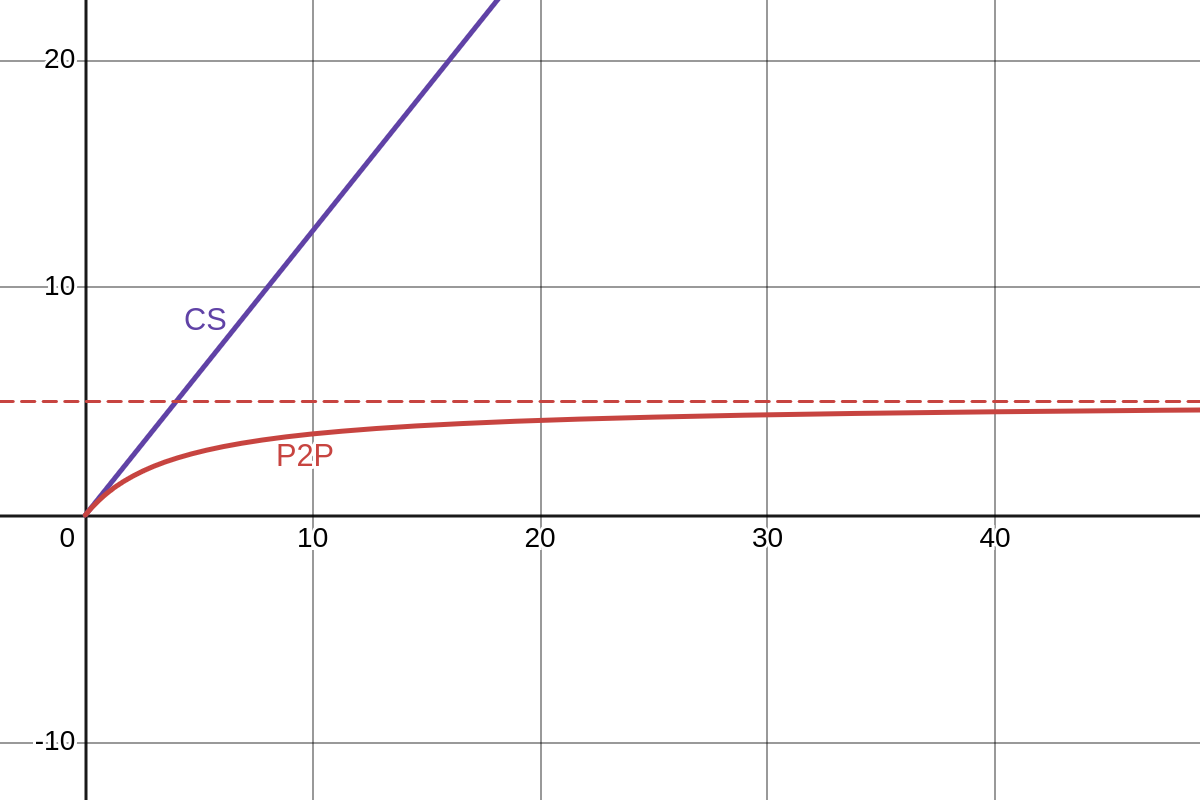
\includegraphics[scale=0.3]{../figures/cs_p2p_ft.png}
\end{center}
\end{minipage}

\subsection{Protocollo BitTorrent}
Approfondiamo le reti P2P, e le \textit{overlay network}, studiando un protocollo reale: il \textbf{protocollo BitTorrent}.

In BitTorrent non è previsto un server centrale che distribuisce il file.
Ogni file è diviso in più \textbf{chunk}, solitamente di 256 KiB ciascuno.

Un \textbf{torrent} è un gruppo di peer che si impegnano a scambiarsi chunk di un file.
Un server più o meno centralizzato detto \textbf{tracker} traccia i peer che partecipano ad un torrent.

\begin{itemize}
	\item 
Quando un utente vuole scaricare un file, chiede al tracker la lista dei peer che partecipano al torrent dedicato a quel file.
Solitamente questo è un \textit{metafile} che contiene l'IP del tracker, a cui si può quindi richiedere il torrent vero e proprio. 

	\item
I peer che l'utente riceve vengono detti \textbf{vicini}: sono connessi da una connessione TCP, e possono quindi scambiarsi dei messaggi (chunk del file).
Possiamo definire così gli utenti collegati ad un torrent:
\begin{itemize}
	\item \textbf{Leecher}: (\textit{"sanguisughe"}), non hanno una copia completa del file e lo stanno ancora scaricando;
	\item \textbf{Seeders}: (\textit{"alimentatori"}), hanno già il file, e lo rendono disponibile agli altri.
\end{itemize}

	\item
Il trasferimento da seeder a leecher si fa un chunk per volta, adottando una politica \textbf{Rarest-First} (\textit{RF}): si inizia a scaricare dal chunk che meno peer sul torrent hanno disponibile. Questo è chiaramente mirato a ottenere i chunk che potrebbero sparire dalla rete il prima possibile.

La lista dei chunk disponibili è fatta richiedendo periodicamente a ogni peer quali chunk possiedono.

	\item 
		Man di mano che i leecher ottengono chunk, devono anche iniziare a rimetterli nella rete ai leecher nuovi arrivati. Su BitTorrent si usa la politica \textbf{Tit for Tat} (\textit{TT}): si inviano chunk ai 4 peer che ci stanno inviando chunk a frequenza più alta.
		Questi top 4 vengono ricalcolati ogni 10 secondi, e gli altri vengono \textit{"strozzati"} (non più serviti).

		Questo significa che i peer potrebbero legarsi eccessivamente fra di loro: ogni 30 secondi si sceglie allora un'altro peer a caso, facendo una previsione \textit{ottimistica} (quel peer potrebbe arrivare fra i nuovi top 4 più frequenti).

		In ogni caso, l'obiettivo è quello di trovare buoni partner per il trasferimento file, in modo da ottenere il file più velocemente possibile.
\end{itemize}

La politica \textit{Tit for Tat} di BitTorrent è chiaramente pensata per scoraggiare i \textit{freeloader}: non si può scaricare se non si dà qualcosa in cambio, cioè si partecipa attivamente al trasferimento rimettendo chunk in circolo.

\subsection{Streaming video e CDN}
Vediamo come si possono creare tecnologie per il trasferimento massiccio di contenuti multimediali, con riferimento allo \textbf{streaming video} e i \textbf{CDN} (\textit{Content Distribution Networks}).

I problemi sono la \textbf{scala} (come raggiungere molti utenti?) e l'\textbf{eterogeneità} (diversi utenti hanno diverse caratteristiche di trasmissione, dispositivi di visualizzazione, ecc...).

La soluzione è infrastruttura \textbf{distribuita} al livello application.

\subsubsection{Video}
Un \textbf{video} è una sequenza di immagini dette \textbf{frame} mostrate a frequenza costante (standard 24, 30, e 60 \textbf{FPS} (\textit{Frames Per Second})).
Un \textbf{frame} è un'array di pixel, dove ogni pixel è rappresentato da 3 valori (corrispondenti ai colori primari additivi \textit{rosso}, \textit{verde} e \textit{blu}).

La tecnica del \textbf{coding} consiste nell'usare ridondanza intrinseca dentro e fra i frame per ridurre i bit usati nel processo di codifica:
\begin{itemize}
	\item Si usa la correlazione \textbf{spaziale}, dentro i singoli frame;
	\item Si usa la correlazione \textbf{temporale}, fra diversi frame.
\end{itemize}

Esistono più tipi di coding, fra cui notiamo:
\begin{itemize}
	\item \textbf{CBR} (\textit{Constant Bit Rate}), a bitrate costante;
	\item \textbf{VBR} (\textit{Variable Bit Rate}), a bitrate variabile;
\end{itemize}

\subsubsection{Streaming}
Lo \textbf{streaming} di video allocati in remoto consiste nel spedire contenuti video abbastanza velocemente da renderli disponibile in \textit{tempo reale} (a differenza del semplice download, che prevede una fase iniziale di acquisizione e una seconda fase di visualizzazione quando il file è ormai già tutto sul disco locale).

Il server dovrà quindi inviare al client frame con una frequenza prefissata (quella del contenuto video), e il client potrà mostrarli appena arrivati.
Assunta una rete ideale, quindi a ritardo \textit{costante}, questo ci permetterebe di visualizzare il video così com'è (al pari di tale ritardo costante).

Purtroppo la rete non è ideale, e il ritardo è quindi \textit{variabile} nel tempo.
Possiamo quindi sfruttare il processo del \textbf{buffering}: aspettiamo un po' lato client prima di mostrare i frame (per un tempo detto \textit{client playout delay}), mettendoli nel frattempo in un \textit{buffer} di memoria.
Quando iniziamo a visualizzare i frame, ci aspettiamo che il buffer sia abbastanza \textit{"pieno"} da permettere la visualizzazione di un segmento di video abbastanza lungo da permettere l'acquisizione dei frame successivi, e così via. 

\end{document}
